\newcommand{\lecturetitle}[1]{
  \title{01204211 Discrete Mathematics \\ #1}
  \author{Jittat Fakcharoenphol}
  \frame{\titlepage}
}
\newcommand{\Mod}{\,\bmod\,}


\newcommand\sbullet[1][.5]{\mathbin{\vcenter{\hbox{\scalebox{#1}{$\bullet$}}}}}

\lecturetitle{Lecture 8b: Finite automa\footnote{Based on lecture notes of {\em Models of Computation} course by Jeff Erikson.}} 
\renewcommand{\epsilon}{\varepsilon}

\newcommand{\czero}{{\mathtt 0}}
\newcommand{\cone}{{\mathtt 1}}

\begin{frame}
  \frametitle{Example: syntax highlighting}
\end{frame}

\begin{frame}
  \frametitle{HTML tokenizer}
\end{frame}

\begin{frame}
  \frametitle{Game programming}
\end{frame}

\begin{frame}
  \frametitle{State-transition graphs}
\end{frame}

\begin{frame}
  \frametitle{More examples over $\Sigma=\{\czero,\cone\}$}
  All strings, except $\czero\cone\czero$.
  \vspace{1in}

  Strings containing the subsequence $\czero\cone\czero$.
  \vspace{1in}
\end{frame}

\begin{frame}
  \frametitle{Formal definitions}

  A {\color{red}\bf finite-state machine} or a {\color{red}\bf
    deterministic finite-state automaton} (DFA) has five components:

  \pause

  \begin{itemize}
  \item the input alphabet $\Sigma$, \pause
  \item a finite set of states $Q$, \pause
  \item a transition function $\delta$ \pause $:Q\times\Sigma \longrightarrow Q$ \pause
  \item a start state $s\in Q$, and
  \item a subset $A\subseteq Q$ of accepting states.
  \end{itemize}
  
\end{frame}

\begin{frame}
  \frametitle{Example 1}

  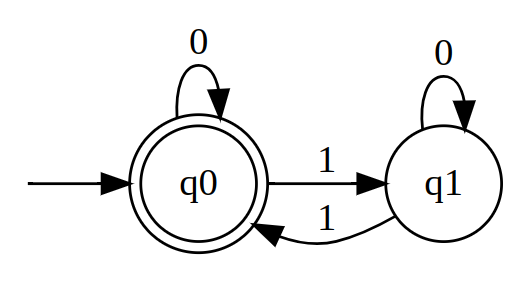
\includegraphics[width=2in]{images/gv/mc02-fa-ex1.png}
\end{frame}

\begin{frame}
  \frametitle{Example 2}

  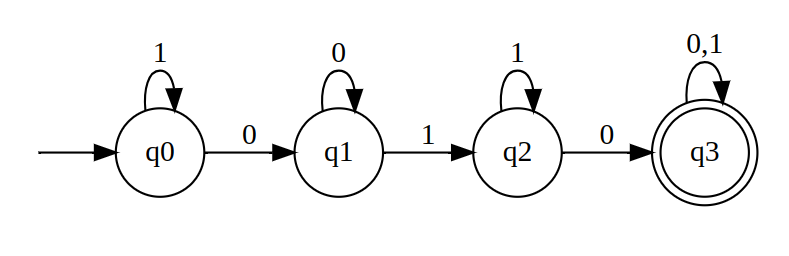
\includegraphics[width=3in]{images/gv/mc02-fa-ex2.png}
\end{frame}

\begin{frame}
  \frametitle{Moves}

  {\bf One step move}: from state $q$ with input symbol $a$, the
  machine changes its state to \pause $\delta(q,a)$.

  {\bf Extension:} from state $q$ with input string $q$, the machine
  changes its state to $\delta^*(q,w)$ defined as

  \pause

  \begin{block}{}
  \[
  \delta^*(q,w) = \left\{
  \begin{array}{ll}
    q & \mbox{if $w=\epsilon$,} \\
    \delta^*(\delta(q,a),x) & \mbox{if $w=ax$.}
  \end{array}
  \right.
  \]
  \end{block}
  
  The signature of $\delta^*$ is $Q\times\Sigma^* \longrightarrow Q$.
\end{frame}

\begin{frame}
  \frametitle{Acceptance}

  For a finite-state machine with starting state $s$ and accepting
  states $A$, it accepts string $w$ iff

  \pause

  \[
  \delta^*(s,w)\in A.
  \]
  
\end{frame}

\begin{frame}
  \frametitle{Digital design: Implementation}

\end{frame}

\begin{frame}
  \frametitle{Digital design: Moore and Mealy machines}

  In the digital design class, you will encounter finite-state
  machines as well.  The version we consider in this class is refered
  to as a {\bf Moore machine}.

  In practices, there is another variant of FSM called {\bf Mealy
    machines}, whose outputs depend on input symbols as well.

  \pause

  Formally, they differ in output function.

  \begin{itemize}
  \item Moore machine: $G:Q \longrightarrow [0,1]$
  \item Mealy machine: $G:Q\times \Sigma \longrightarrow [0,1]$
  \end{itemize}
  
\end{frame}
